
\section{The Complex Fourier Basis}

\par \indentt Because the real Fourier series employs sines and cosines, its connection to sound waves is clear and intuitive. However, it is impractical to work with. For one thing, the coefficients can only be derived by calculating three different inner products. For another, the terms of the real Fourier basis $\DNT$ are given in a peculiar order and cannot be elegantly made into a vector. Finally, though $\DNT$ is orthogonal,\footnote{In the interest of getting to the good stuff, the orthogonality of $\DNT$ will not be proved in this paper. It would proceed much like the upcoming Lemma \ref{lem:complex_F_is_ortho}.} it is not orthonormal. 

\par \bigskip We solve all these problems by using the complex Fourier basis $\FNT$. Its coefficients can be calculated with one inner product, and its terms neatly correspond to a vector of length $2N+1$. Most importantly, as I will prove, $\FNT$ is orthonormal under the complex inner product defined in \ref{defn:complex_innerprod}.

\begin{definition}{The $N$'th-order complex Fourier basis is the set of pure tones with frequency $\frac{n}{T}$ where $-N\le n \le N$, notated as}
    \[\mathcal{F}_{N,T}= \left\{\begin{array}{ll}
   e^{-\frac{2\pi iNt}{T}},e^{-\frac{2\pi i(N-1)t}{T}}, ..., e^{-\frac{2\pi it}{T}}, \\
   1,e^{\frac{2\pi it}{T}}, ..., e^{\frac{2\pi i(N-1)t}{T}}, e^{\frac{2\pi iNt}{T}}
   \end{array}\right\}.\cite{Ryan}
   \]
   \label{defn:complex_F_basis}
\end{definition}

\par To show that $\FNT$ spans $\VNT$ just as $\DNT$ does, we take advantage of Euler's Formulas, swapping in $\frac{2\pi nt}{T}$ as the continuous variable:

\begin{definition}
    Euler's Formulas are\\
    
    $\puretone{nt}{T} = \cos\bigg(\frac{2\pi nt}{T}\bigg)+i\sin\bigg(\frac{2\pi nt}{T}\bigg)$ \hspace{.3in} and \hspace{.3in} $e^{-\frac{2\pi int}{T}} = \cos\bigg(\frac{2\pi nt}{T}\bigg)-i\sin\bigg(\frac{2\pi nt}{T}\bigg)$.
\end{definition}

\newpage 

\par These equations allow us to turn the cosine terms of the real Fourier series into complex exponential terms:\\

\indentt $\cos(\frac{2\pi nt}{T}) = \puretone{nt}{T} - i\sin(\frac{2\pi nt}{T}) = \puretone{nt}{T} + e^{-\frac{2\pi int}{T}} - \cos(\frac{2\pi nt}{T})$

\indentt $2\cos(\frac{2\pi nt}{T}) = \puretone{nt}{T} + e^{-\frac{2\pi int}{T}}$

\indentt $\cos(\frac{2\pi nt}{T}) = \frac{1}{2} (\puretone{nt}{T} + e^{-\frac{2\pi int}{T}})$\\

\par The sine terms become complex exponential terms as well:\\

\indentt $\sin(\frac{2\pi nt}{T}) = \frac{1}{i} (\puretone{nt}{T} - \cos(\frac{2\pi nt}{T})) = \frac{1}{i} (\puretone{nt}{T} - e^{-\frac{2\pi int}{T}}) - \sin(\frac{2\pi nt}{T})$

\indentt $2\sin(\frac{2\pi nt}{T}) = \frac{1}{i} (\puretone{nt}{T} + e^{-\frac{2\pi int}{T}})$

\indentt $\sin(\frac{2\pi nt}{T}) = \frac{1}{2i} (\puretone{nt}{T} + e^{-\frac{2\pi int}{T}})$\\

\par Therefore, since $\DNT$ spans $\VNT$, $\FNT$ must also span $\VNT$. Definition \ref{defn:complex_F_series} gives the terms of the $N$'th-order complex Fourier series for some $T$-periodic function.

\begin{definition}{The $N$'th-order complex Fourier series for a function $f(t)$ with period $T$ is}
    $$f_N(t)=\sum_{n=-N}^{N}{c_n \puretone{nt}{T}}.\cite{Ryan}$$
    \label{defn:complex_F_series}
\end{definition}

Finding the complex coefficients $c_n$ is a much simpler task than finding real Fourier coefficients. To do so, we employ an inner product on the space of complex $T$-periodic functions, which uses the complex conjugate $\overline{g(t)}$ of the function $g(t)$. Taking the complex conjugate of a function leaves its real part alone while flipping the sign of its imaginary part. For complex exponentials, the sign of the exponent is flipped, i.e. $\puretone{nt}{T}$ becomes $e^{-\frac{2\pi int}{T}}$.

\begin{definition}{The complex inner product for $T$-periodic functions}
    $$\innerprod{f}{g} = \frac{1}{T} \int_0^T f(t)\overline{g(t)}dt$$
    \label{defn:complex_innerprod}
\end{definition}

\begin{definition}{The coefficients of the complex Fourier series of a function $f(t)$ with period $T$ are given by}
    $$c_n = \innerprod{f}{\puretone{nt}{T}} = \frac{1}{T} \int_0^T f(t)e^{-\frac{2\pi int}{T}}dt.$$
    \label{defn:complex_F_coeffs}
\end{definition}

\par We established earlier that Fourier approximation is a change of basis from the continuous-time domain to the frequency domain. Now we have a way to change the basis in the other direction: simply use the components of the amplitude vector $\{c_{-N},c_{-N+1},...,c_{-1},c_0,c_1,...,c_{N-1},c_N\}$ as the coefficients of $\FNT$ to obtain $f_N(t)$.

\subsection{Orthonormality of the Complex Fourier Basis}

\par \indentt Proving that a basis is orthonormal takes two steps:

\begin{enumerate}
    \item Prove that each vector in the basis is orthogonal to the rest. To do so, show that the inner product of any two different basis vectors is 0.
    \item Prove that each vector in the basis is normal. To do so, show that the inner product of any basis vector with itself is 1.
\end{enumerate}

\par Taken together, Lemmas \ref{lem:complex_F_is_ortho} and \ref{lem:complex_F_is_normal} prove that the complex Fourier basis is indeed orthonormal.\\

\begin{lemma}
    The inner product of any two unique vectors in $\FNT$ is 0.\\
    
    \begin{proof}
        Consider arbitrary $\vecv_1,\vecv_2 \in \FNT$ such that $\vecv_1 \not= \vecv_2$. Then $\vecv_1 = \puretone{n_1t}{T}$ and $\vecv_2 = \puretone{n_2t}{T}$ for some $-N \le n_1,n_2 \le N$ such that $n_1 \not= n_2$. We see that 
        
        \begin{multline*}
            \innerprod{\vecv_1}{\vecv_2} = \frac{1}{T} \int_0^T e^{\frac{2\pi in_1t}{T}}\overline{e^{\frac{2\pi in_2t}{T}}}dt = \frac{1}{T} \int_0^T e^{\frac{2\pi i(n_1-n_2)t}{T}}dt
            = \frac{e^{\frac{2\pi i(n_1-n_2)t}{T}}}{2\pi i(n_1-n_2)T}\Bigg]^T_0 \\= \frac{e^{2\pi i(n_1-n_2)}-1}{2\pi i(n_1-n_2)T}
            = \frac{cos(2\pi (n_1-n_2))+i\sin(2\pi (n_1-n_2))-1}{2\pi i(n_1-n_2)T}
            = \frac{1+i\cdot 0-1}{2\pi i(n_1-n_2)T} = 0.
        \end{multline*}
    \end{proof}
    \label{lem:complex_F_is_ortho}
\end{lemma}

\begin{lemma}
    The inner product of any vector in $\FNT$ with itself is 1.\\
    
    \begin{proof}
        Consider arbitrary $\vecv_0 \in \FNT$. Then $\vecv_0 = \puretone{n_0t}{T}$ for some $-N \le n_0 \le N$. We see that 
        
        \begin{multline*}
            \innerprod{\vecv_0}{\vecv_0} = \frac{1}{T} \int_0^T e^{\frac{2\pi in_0t}{T}}\overline{e^{\frac{2\pi in_0t}{T}}}dt = \frac{1}{T} \int_0^T e^{\frac{2\pi i(n_0-n_0)t}{T}}dt\\
            = \frac{1}{T} \int_0^T e^{0}dt = \frac{1}{T} \int_0^T 1 dt = \frac{t}{T}\bigg]^T_0 = 1.\footnote{This would have come out to $T$ if not for the normalizing factor \frac{1}{T}.}
        \end{multline*}
    \end{proof}
    \label{lem:complex_F_is_normal}
\end{lemma}

\newpage

\par As promised, we will use $\FNT$'s orthonormality to prove its linear independence.

\begin{theorem}
    \par Let arbitrary $\puretone{n_1t}{T},\puretone{n_2t}{T},\dots,\puretone{n_kt}{T}\in\FNT$ for some $k \le N$. Assume $c_1\puretone{n_1t}{T} + c_2\puretone{n_2t}{T} + \dots + c_k\puretone{n_kt}{T} = 0$. Then $c_1 = c_2 = \dots = c_k = 0$. In other words, $\puretone{n_1t}{T},\puretone{n_2t}{T},\dots,\puretone{n_kt}{T}$ are linearly independent.
    
    \begin{proof}
        \par Take the inner product of both sides of $c_1\puretone{n_1t}{T} + c_2\puretone{n_2t}{T} + \dots + c_k\puretone{n_kt}{T} = 0$ with $\puretone{n_jt}{T}$ for some arbitrary $j\in\{1,2,\dots,k\}$.
        
        \par \bigskip On the left, we see that $\innerprod{c_1\puretone{n_1t}{T} + c_2\puretone{n_2t}{T} + \dots + c_k\puretone{n_kt}{T}}{\puretone{n_0t}{T}} = c_1\innerprod{\puretone{n_1t}{T}}{\puretone{n_jt}{T}} + c_2\innerprod{\puretone{n_2t}{T}}{\puretone{n_jt}{T}} + \dots + c_j\innerprod{\puretone{n_jt}{T}}{\puretone{n_jt}{T}} + \dots + c_k\innerprod{\puretone{n_kt}{T}}{\puretone{n_jt}{T}}$. Since $\FNT$ is orthonormal, this expression is equal to $c_1\cdot 0 + c_2\cdot 0 + \dots + c_j\cdot 1 + \dots + c_k\cdot 0 = c_j$.
        
        \par \bigskip On the right, we see that $\innerprod{0}{\puretone{n_jt}{T}} = 0$. Then $c_j = 0$, and since $c_j$ is arbitrary, all the coefficients equal 0.
    \end{proof}
    \label{thm:complex_F_lin_indep}
\end{theorem}

\begin{figure}[h]
    \centering
    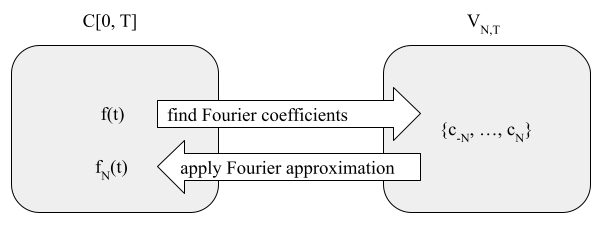
\includegraphics[scale=.5]{real_F_space_diagram.png}
    \caption{Moving between continuous time and the frequency space}
    \label{fig:real_F_space_diagram}
\end{figure}

\par \bigskip Since each of the pure tones in $\FNT$ is linearly independent from the rest, the frequency information of a tone $f$ is completely preserved when taken from the time domain to the frequency domain and back again. Thus, a musician can obtain Fourier coefficients for the $T$-periodic sound function of their choice, modify them, and return the new function to continuous time without eliminating or muddling any of the harmonics, nor changing the pitch.

\par \bigskip Meanwhile, since each pure tone in $\FNT$ is a unit vector, its amplitude is unaffected by changes in coordinates. A musician can alter the amplitudes of harmonic frequencies to their heart's content without worrying about calculating some denominator for each Fourier coefficient when changing bases.

\par \bigskip Now that we have a nice and ergonomic setting to mess around with sound quality, we can finally start discussing how the messing-around is actually accomplished. At long last, the next section mathematically defines filters that operate on continuous-time functions. In this setting, they are called \textbf{analog filters}, while \textbf{digital filters} (discussed later) operate on discrete vectors of sampled amplitudes.